\section{Additional Experimental Tables and Plots}
\label{app:extended}

\subsection{Extended comparator taxonomy}

\begin{center}
\footnotesize
\setlength{\tabcolsep}{2pt}
\begin{longtable}{@{}>{\raggedright\arraybackslash}p{1.58cm}>{\raggedright\arraybackslash}p{1.65cm}>{\raggedright\arraybackslash}p{0.82cm}>{\raggedright\arraybackslash}p{0.92cm}>{\raggedright\arraybackslash}p{0.88cm}>{\raggedright\arraybackslash}p{1.0cm}>{\raggedright\arraybackslash}p{3.08cm}@{}}
\caption{Extended comparator taxonomy used to frame the project.}\label{tab:taxonomy}\\
\toprule
Method & Mech. & Q? & Access & Bound & Stat. & Caveat \\
\midrule
\endfirsthead
\toprule
Method & Mech. & Q? & Access & Bound & Stat. & Caveat \\
\midrule
\endhead
Full KV & Exact cache & No & Exact & Exact & Proj. & No compression or skipping \\
INT8 & Uniform quantization & No & Yes & No & Proj. & Keeps all entries \\
KIVI & Asymmetric low-bit quantization & No & Yes & No & KIVI-st. & Project approximation \\
SnapKV & Window-based token selection & Yes & Ltd. & No & Snap-st. & Discards positions \\
Quest & Query-aware page retrieval & Yes & Page-level & No & Quest-st. & Discrete budget match \\
H2O & Heavy-hitter eviction & Yes & Ltd. & No & Lit. & Eviction-focused \\
Ada-KV & Adaptive budget allocation & Yes & Ltd. & No & Lit. & No local certificate \\
DeltaKV & Residual-style compression & No & Ltd. & No & Lit. & Compression overlap \\
OjaKV & Online low-rank compression & No & Ltd. & No & Lit. & Different approximation family \\
ClusterKV & Semantic clustering & Yes & Ltd. & No & Lit. & Retrieval by clustering \\
EchoKV & Similarity reconstruction & No & Ltd. & No & Lit. & No skip theorem \\
PL tries & Predictive coding & Impl. & No & No & Lit. & Poor random access \\
PagedAttn. & Paging and serving & No & Yes & No & Lit. & Systems-only \\
RACK-KV & Block-local compression plus certificate & Yes & Yes & Yes & Proj. & Local theorem only \\
\bottomrule
\end{longtable}
\end{center}


\subsection{Longer-prompt layer-0 pilot}

The longer supporting pilot fixes \(W=16\) and \(B=8\) and varies only the skip tolerance. Its purpose is modest: to test the chosen configuration on a 256-token layer-0 trace, not to claim a complete hyperparameter sweep.

\begin{table}[h]
  \centering
  \small
  \begin{threeparttable}
\begin{tabular}{@{}c
S[table-format=2.0]
S[table-format=2.0]
S[table-format=1.2]
S[scientific-notation=true,table-format=1.2e-1]
S[scientific-notation=true,table-format=1.2e-1]@{}}
\toprule
Tolerance & {Cases} & {Certified skips} & {Skip fraction (\%)} & {Max observed error} & {Max bound} \\
\midrule
0.00 & 66 & 0 & 0.00 & 0 & 0 \\
0.01 & 66 & 3 & 0.22 & 2.10e-3 & 4.12e-3 \\
0.05 & 66 & 3 & 0.22 & 2.10e-3 & 4.12e-3 \\
0.10 & 66 & 3 & 0.22 & 2.10e-3 & 4.12e-3 \\
\bottomrule
\end{tabular}
\end{threeparttable}

  \caption{Supporting 256-token layer-0 pilot across four tolerances. Certified skips appear only at nonzero tolerances, and the skip fraction remains small.}
  \label{tab:pilot}
\end{table}

\begin{figure}[h]
  \centering
  \begin{tikzpicture}
\begin{axis}[
  width=0.98\linewidth,
  height=6.0cm,
  xlabel={Tolerance},
  ylabel={Weighted certified skip fraction (\%)},
  xmin=-0.005,
  xmax=0.105,
  ymin=0,
  ymax=0.26,
  grid=both,
  major grid style={gray!20},
  minor grid style={gray!10},
  tick label style={font=\small},
  label style={font=\small}
]
  \addplot[mark=*, mark size=2pt, color=blue!70!black, thick]
    table[
      col sep=comma,
      x=tolerance,
      y expr=\thisrow{weighted_skipped_block_fraction}*100
    ]{data/stage2b_tolerance_summary.csv};
\end{axis}
\end{tikzpicture}

  \caption{Weighted certified skip fraction versus tolerance in the supporting 256-token layer-0 pilot. The curve rises immediately from zero and then plateaus because the same three blocks are certified at all nonzero tolerances tested.}
  \label{fig:skipvstol}
\end{figure}

\subsection{Serialized-byte structure}

\begin{table}[h]
  \centering
  \small
  \begin{threeparttable}
\begin{tabular}{@{}l
S[table-format=2.1]
S[table-format=2.1]
S[table-format=1.2]
S[table-format=1.2]
S[table-format=1.2]
S[table-format=2.1]@{}}
\toprule
Method & {Keys (kB)} & {Values (kB)} & {Scales} & {Meta + index} & {Recent} & {Total (kB)} \\
\midrule
RACK-KV & 23.4 & 23.4 & 0.08 & 1.12 & 8.19 & 56.2 \\
Uniform INT8 & 20.8 & 20.8 & 0.65 & 0.88 & 8.19 & 51.3 \\
SnapKV-style (matched) & 23.5 & 23.5 & 0.00 & 1.03 & 8.19 & 56.2 \\
Quest-style (matched) & 23.5 & 23.5 & 0.00 & 1.02 & 8.19 & 56.2 \\
KIVI-style & 5.2 & 5.2 & 1.16 & 1.06 & 8.19 & 20.8 \\
\bottomrule
\end{tabular}
\end{threeparttable}

  \caption{Mean serialized-byte breakdown in the representative-layer benchmark. Metadata overhead explains why RACK-KV uses slightly more bytes than uniform INT8 even though its reconstruction error is lower.}
  \label{tab:storagebreakdown}
\end{table}

\begin{figure}[h]
  \centering
  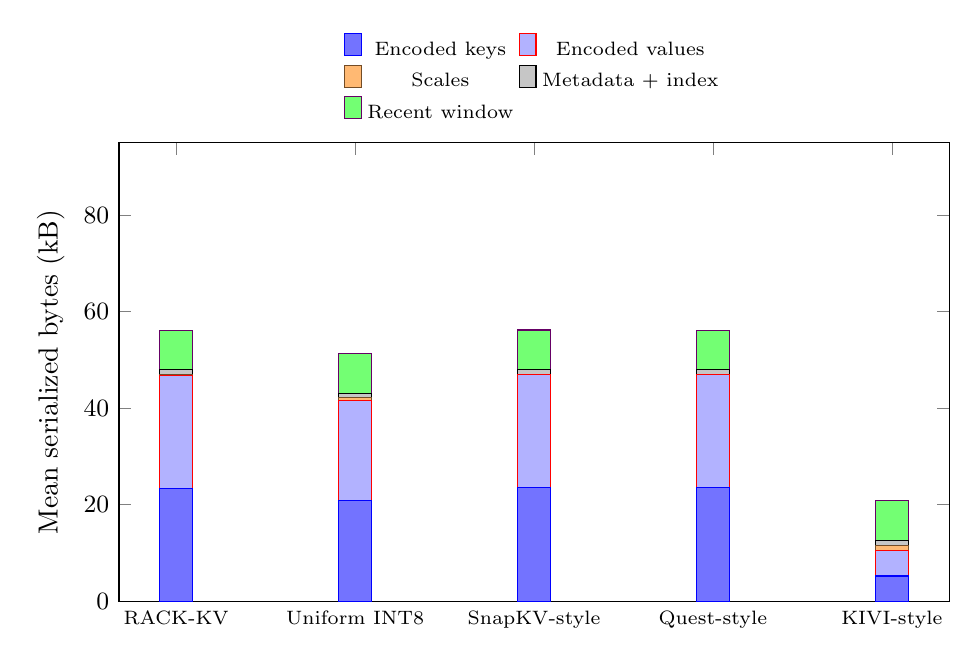
\begin{tikzpicture}
\begin{axis}[
  width=\linewidth,
  height=7.4cm,
  ybar stacked,
  bar width=12pt,
  ymin=0,
  ymax=95,
  ylabel={Mean serialized bytes (kB)},
  symbolic x coords={RACK-KV,Uniform INT8,SnapKV-style,Quest-style,KIVI-style},
  xtick=data,
  xticklabel style={font=\scriptsize, align=center},
  yticklabel style={font=\small},
  legend style={draw=none, fill=none, font=\scriptsize, legend columns=2, at={(0.5,1.02)}, anchor=south},
  nodes near coords={},
  enlarge x limits=0.08
]
  \addplot+[fill=blue!55] coordinates {(RACK-KV,23.40) (Uniform INT8,20.78) (SnapKV-style,23.49) (Quest-style,23.48) (KIVI-style,5.20)};
  \addplot+[fill=blue!30] coordinates {(RACK-KV,23.40) (Uniform INT8,20.78) (SnapKV-style,23.49) (Quest-style,23.48) (KIVI-style,5.20)};
  \addplot+[fill=orange!55] coordinates {(RACK-KV,0.08) (Uniform INT8,0.65) (SnapKV-style,0.00) (Quest-style,0.00) (KIVI-style,1.16)};
  \addplot+[fill=gray!45] coordinates {(RACK-KV,1.12) (Uniform INT8,0.88) (SnapKV-style,1.03) (Quest-style,1.02) (KIVI-style,1.06)};
  \addplot+[fill=green!55] coordinates {(RACK-KV,8.19) (Uniform INT8,8.19) (SnapKV-style,8.19) (Quest-style,8.19) (KIVI-style,8.19)};
  \legend{Encoded keys,Encoded values,Scales,Metadata + index,Recent window}
\end{axis}
\end{tikzpicture}

  \caption{Stacked byte categories for representative-layer methods. RACK-KV spends bytes on anchors, scales, and indexing to preserve independent random access.}
  \label{fig:storagebreakdown}
\end{figure}

\subsection{Position dependence}

\begin{figure}[h]
  \centering
  \begin{tikzpicture}
\begin{axis}[
  width=0.98\linewidth,
  height=6.2cm,
  xlabel={Query position},
  ylabel={Mean attention-output L2 error},
  xmin=31,
  xmax=255,
  ymin=0,
  ymax=0.0055,
  grid=both,
  major grid style={gray!20},
  minor grid style={gray!10},
  tick label style={font=\small},
  label style={font=\small}
]
  \addplot[mark=*, mark size=1.6pt, color=blue!70!black, thick]
    table[col sep=comma, x=query_position, y=mean_attention_output_l2_error]{data/stage4_rack_by_position.csv};
\end{axis}
\end{tikzpicture}

  \caption{Mean RACK-KV local attention-output error versus query position in the representative-layer benchmark. The error is not monotone in position, although the serialized cache size increases steadily with the visible prefix.}
  \label{fig:errorposition}
\end{figure}

\subsection{Verified full-model status}

As of Sunday, July 26, 2026, the local evidence shows that a full 32-layer teacher-forced evaluation framework exists, but a verified final package for the full-model run is not yet complete. Accordingly, the paper reports no final-model quality numbers.
